\documentclass[11pt]{article}
\usepackage[margin=1in]{geometry} 
\usepackage{amsmath,amsthm,amssymb,amsfonts}

\usepackage{mathpazo}
\usepackage{euler}
\usepackage{xcolor}
\usepackage{tikz}
\usetikzlibrary{matrix}
\usepackage{fancyhdr}
\pagestyle{fancy}

\newcommand{\N}{\mathbb{N}}
\newcommand{\Z}{\mathbb{Z}}
\newcommand{\Q}{\mathbb{Q}}
\newcommand{\R}{\mathbb{R}}
\newcommand{\C}{\mathbb{C}}
\newcommand{\M}[2]{\mathsf{M}_{#1}#2}
\newcommand{\im}{\operatorname{im}}
\newcommand{\eps}{\varepsilon}
\newcommand{\dpart}[2]{\frac{\partial#1}{\partial#2}}
\newcommand{\nat}[1]{[\![#1]\!]}
\newcommand{\natzero}[1]{\nat{#1}_0}
\newcommand{\adj}[1]{\operatorname{adj}(#1)}
\newcommand{\ip}[2]{\langle #1 , #2 \rangle}
\newcommand{\paint}[2]{\color{#1}{#2}}
\definecolor{purple}{RGB}{129, 0, 125}

\renewcommand*{\proofname}{\paint{purple}{Demostraci\'on}}
\newenvironment{theorem}[2][Teorema]{\begin{trivlist}
\item[\hskip \labelsep {\bfseries #1}\hskip \labelsep {\bfseries #2.}]}{\end{trivlist}}
\newenvironment{lemma}[2][Lema]{\begin{trivlist}
\item[\hskip \labelsep {\bfseries #1}\hskip \labelsep {\bfseries #2.}]}{\end{trivlist}}
\newenvironment{exercise}[2][Ejercicio]{\begin{trivlist}
\item[\hskip \labelsep \paint{purple}{{\bfseries #1}}\hskip \labelsep {\bfseries #2.}]}{\end{trivlist}}
\newenvironment{reflection}[2][Resoluci\']{\begin{trivlist}
\item[\hskip \labelsep {\bfseries #1}\hskip \labelsep {\bfseries #2.}]}{\end{trivlist}}
\newenvironment{proposition}[2][Proposici\'on]{\begin{trivlist}
\item[\hskip \labelsep {\bfseries #1}\hskip \labelsep {\bfseries #2.}]}{\end{trivlist}}
\newenvironment{corollary}[2][Corolario]{\begin{trivlist}
\item[\hskip \labelsep {\bfseries #1}\hskip \labelsep {\bfseries #2.}]}{\end{trivlist}}

%-----------------------

\title{
\LARGE{\paint{purple}{Geometr\'ia Diferencial}}
\\
\vspace{0.5pt}
\small{\paint{purple}{Ejercicios para Entregar - Pr\'actica 1}}
}
\author{\paint{purple}{Guido Arnone}}
\date{}
\lhead{Guido Arnone}
\rhead{Pr\'actica 1}

\begin{document}

\maketitle
\begin{exercise}{4} Probar que:
\begin{itemize}
\item[(a)] El conjunto de vectores normales unitarios a una curva regular en $\R^3$ tiene una estructura natural de variedad diferenciable de dimensi\'on $2$.
\item[(b)] Sea $\Omega$ un abierto de $\R^n$ y sea $F : \Omega \to \R$ una función diferenciable que tiene a $0$ como valor regular, de manera que el conjunto $M = F^{-1}(0)$ es una subvariedad
de $\R^n$. Muestre que el conjunto $SM$ de vectores unitarios tangentes a $M$ tiene una estructura natural de variedad de dimensi\'on $2n - 3$.
\end{itemize}
\end{exercise}
\begin{proof}
\hspace{0.5pt}
\begin{itemize}
\item[(a)] Sea $\alpha : I \to \mathcal{C}$ una parametrizaci\'on $\mathcal{C}^2$ de una curva regular de curvatura positiva y, sin p\'erdida de generalidad, la suponemos parametrizada por longitud de arco. Ahora, dado un punto $p = \alpha(t_0)$ en la traza, la recta tangente a la curva all\'i es $L_p = \{\lambda \alpha'(t_0) + \alpha(t_0)\}$. Ahora, los vectores normales unitarios a $\mathcal{C}$ en $p$ son los vectores normales unitarios a $L_p$ en $p$, los cuales se pueden describir como
\begin{align*}
\mathcal{N}_p := \{v \in \R^3 : \ip{\alpha'(t_0)}{v} = 0, \ip{v}{v} = 1 \}.
\end{align*}
Consideramos entonces
\begin{align*}
\mathcal{N} = \{(t,v) : \ip{\alpha'(t)}{v} = 0, \ip{v}{v} = 1\}
\end{align*}
Veamos que \'esta es una variedad diferenciable de dimensi\'on $2$. Notemos que $\mathcal{N}$ es la preimagen del $(0,1)$ por la siguiente funci\'on
\begin{align*}
F : \R^4& = \R \times \R^3 \mapsto \R^2 \\
& (t,v) \mapsto (\ip{\alpha'(t)}{v},\ip{v}{v})
\end{align*}
que es diferenciable, pues $\alpha \in \mathcal{C}^2(I)$. Por el teorema de valores regulares, bastar\'ia probar que $DF_p$ es sobreyectivo para cada $p \in F^{-1}(0,1)$. Como
\begin{align*}
DF_{(t,v)} = \begin{pmatrix}
\ip{\alpha''(t)}{v} & \alpha'(t) \\
0 & 2v
\end{pmatrix},
\end{align*}
esto es equivalente a que las filas no sean m\'ultiplos una de la otra. Si fuera as\'i, en particular existir\'ia $\mu \in \R \setminus \{0\}$ tal que $v = \mu \alpha'(t)$ y entonces ser\'ia
\begin{align*}
1 = \ip{v}{v} = \mu \ip{\alpha'(t)}{v} = 0
\end{align*}
lo que es absurdo. En conclusi\'on, necesariamente las filas de $D_pF$ son linealmente independientes (i.e. el diferencial es sobreyectivo) cuando $F(p) = (0,1)$, y consecuentemente el teorema de valores regulares asegura que $\mathcal{N}$ es una variedad de dimensi\'on $\dim \mathcal{N} = \dim \R^4 - \dim \R^2 = 2$.
\item[(b)] Buscamos en alg\'un sentido generalizar la idea de $\paint{purple}{(a)}$. Dada $M = F^{-1}(0)$ variedad con $0$ valor regular de $F$, definimos
\begin{align*}
SM := \{(p,v) : p \in M, \ip{\nabla_pF}{v} = 0, \ip{v}{v} = 1\} \subset \R^n \times \R^n = \R^{2n}
\end{align*}
de forma que $SM = \Gamma^{-1}(0,0,1)$ con
\begin{align*}
\Gamma : \ &\R^n \times \R^n \to \R^3 \\
&(p,v) \longmapsto (F(p),\ip{\nabla_pF}{v},\ip{v}{v})
\end{align*}
que es diferenciable pues $F$ y el producto interno lo son. Ahora dado $(p,v) \in SM$, como
\begin{align*}
D\Gamma_{(p,v)} = \begin{pmatrix}
\nabla_pF & 0\\
H & \nabla_pF\\
0 & 2v
\end{pmatrix}
\end{align*}
con $\R^n \ni H = \left(\sum_i\dpart{F}{x_jx_i}(p)v_i\right)_j$ y $\nabla_pF \neq 0$ pues $F(p) = 0$, existe $i \in \nat{n}$ tal que $\dpart{F}{X_i} \neq 0$ y el menor que resulta de quitar la fila $1$ y columna $i$ es de la forma
\begin{align*}
DF_{(p,v)}^{(1,i)} = \begin{pmatrix}
* & \nabla_pF \\
0 & 2v
\end{pmatrix}
\end{align*}
Por el mismo argumento que en $\paint{purple}{(a)}$ este resulta de rango $2$, pues $\nabla_pF \perp v$ y $\nabla_pF,v \neq 0$. Como $D_{(p,v)}F^{(1,i)}$ tiene rango $2$ y la primera fila es linealmente independiente de las siguientes, vemos que $D_{(p,v)}F$ tiene rango $3$ y como este es el m\'aximo, es sobreyectivo. El teorema de valores regulares nos permite entonces concluir que $SM = \Gamma^{-1}(0,0,1)$ es variedad diferenciable y
\begin{align*}
\dim SM = \dim \R^{2n} - \dim \R^3 = 2n-3.
\end{align*}
\end{itemize}
\end{proof}

\begin{exercise}{5} Muestre que los siguientes espacios son variedades diferenciales y determine sus
dimensiones. 
\begin{itemize}
\item[(i)] $\mathsf{SL}(n,\C)$ el conjunto de las matrices complejas de $n \times n$ y determinante $1$.
\item[(ii)] $\mathsf{U}(n,\R) \subset \M{n}{\C}$, el conjunto de las matrices complejas de $n \times n$ que son unitarias, esto es, las matrices $A$ tales que $AA^* = I$.
\item[(iii)] $\mathsf{Sp}(2n,\R)$, el conjunto de las matrices $A \in \mathsf{M}_{2n}\R$ tales que $A\Omega A^t=\Omega$, con
\begin{align*}
  \Omega=\begin{pmatrix}0&I_n\\-I_n&0\end{pmatrix}
\end{align*}
\end{itemize}
\end{exercise}
\begin{proof} Hacemos cada caso por separado.
\begin{itemize} 
\item[(i)] Afirmamos primero que la funci\'on $\det : \M{n}{\C} \to \C$ es diferenciable. Eso es porque dada una matriz compleja $A = (X_{kl}+iY_{kl})_{kl}$, luego $\det A$ es un polinomio con coeficientes en $\C$ en funci\'on de cada $X_{kl}$ e $Y_{kl}$,
\begin{align*}
\det((X_{kl}+iY_{kl})_{i,j}) = \sum_{\sigma \in \mathbb{S}_n}sgn(\sigma)(X_{1\sigma(1)}+iY_{1\sigma(1)}) \cdots (X_{n \sigma(n)}+iY_{n\sigma(n)}).
\end{align*}
Identificando $\M{n}{\C} \equiv \R^{2n^2}$ y $\C \equiv \R^2$, el determinante en cada coordenada (es decir, tomando partes real e imaginaria) resulta un polinomio, y por lo tanto es diferenciable. As\'i, podemos utilizar el teorema de valores regulares pensando $\det$ como una funcion $\R^{2n^2} \to \R^2$ y tomando la preimagen de $(1,0) = 1+0i$ pues por definici\'on es $\mathsf{SL}(n,\C) = \det^{-1}(\{1\})$. Con la intenci\'on de alivianar la notaci\'on seguimos escribiendo $X+iY = (X,Y) \in \R^2$ y de igual forma en $\R^{2n^2}$. Para conocer el diferencial $D := D(\det)$, por linealidad podemos calcularlo en cada direcci\'on can\'onica $E_{kl}$ e $iE_{kl}$, siendo \'estas las $2n^2$-uplas can\'onicas que tienen un $1$ exactamente en el lugar $X_{kl}$ e $Y_{kl}$ respectivamente. Dado $t \in \R$ y usando el desarrollo por cofactores,
\begin{align*}
\det(A+tE_{kl}) &= \sum_{s=1}^n(-1)^{k+s}(A+tE_{kl})_{ks}(A+tE_{kl})^{(k,s)} = \sum_{s=1}^n(-1)^{k+s}(A+tE_{kl})_{ks}A^{(k,s)} \\ 
&= \sum_{s=1}^n(-1)^{k+s}A_{ks}A^{(k,s)} + t(-1)^{k+l}A^{(k,l)} = \det(A) + t(-1)^{k+l}A^{(k,l)}\\
& = \det(A) + t\adj{A}_{kl}
\end{align*}
y del mismo modo, $\det(A+tiE_{kl}) = \det(A) + ti\adj{A}_{kl}$. Por lo tanto,
\begin{align*}
D_A(E_{ij}) = \lim_{t \to 0} \frac{\det(A+tE_{ij}) - \det(A)}{t} = \lim_{t \to 0}\frac{\det(A)+t\adj{A}_{kl}-\det(A)}{t} = \adj{A}_{kl}
\end{align*}
y $D_A(iE_{ij}) = i\adj{A}_{kl}$. Por lo tanto, si $\adj{A}_{kl} = R_{kl} + iI_{kl}$ para cada $k,l \in \nat{n}$ entonces $i\adj{A}_{kl} = iR_{kl} - I_{kl}$ y la matriz diferencial de $\det$ en $A$ como funci\'on $\R^{2n^2} \to \R^2$ es
\begin{align*}
D_A = \begin{pmatrix}
R_{11} & R_{12} & \dots & R_{1n} & R_{21} & \dots & R_{nn} & -I_{11} & \dots & -I_{nn} \\
I_{11} & I_{12} & \dots & I_{1n} & I_{21} & \dots & I_{nn} & R_{11} & \dots & R_{nn}
\end{pmatrix}.
\end{align*}
Si $D_A$ no fuera sobreyectivo, entonces o bien $D_A = 0$ o bien $D_A$ es de rango $1$. Veamos que esto \'ultimo (tambi\'en) implica $\adj{A} = 0$. En efecto, si $\operatorname{rg} D_A = 1$ entonces las filas del diferencial son linealmente dependientes y en consecuencia, existe $\lambda \neq 0$ tal que 
\begin{align*}
\begin{cases}
\quad R_{kl} = \lambda I_{kl}\\
- \ I_{kl} = \lambda R_{kl}
\end{cases}
\end{align*}
para cada $k,l \in \nat{n}$. De aqu\'i concluimos que $R_{kl} = - \lambda^2 R_{kl}$ y por lo tanto $R_{kl}(1+\lambda^2) = 0$ as\'i que $R_{kl} = 0$ e $I_{kl} = -\lambda R_{kl} = 0$. Ahora bien, si $A \in \mathsf{SL}(n,\C)$ luego es
\begin{align*}
I = 1 \cdot I = \det(A) I = A \adj{A},
\end{align*}
y no puede ser entonces $\adj{A} = 0$. En consecuencia, $D_A$ siempre es sobreyectivo cuando $A$ es un elemento de $\mathsf{SL}(n,\C)$ y por lo tanto, el teorema de valores regulares nos asegura que esta \'ultima es variedad diferenciable de dimensi\'on $2n^2 - 2 = 2(n^2-1)$.
\item[(ii)] Con la misma idea que antes identificamos $\M{n}{\C} \equiv \R^{2n^2}$ para usar el teorema de valores regulares. Notemos que dada cualquier matriz $A$ luego $AA^* -I$ es siempre Hermitiana y podemos considerar entonces la funci\'on
\begin{align*}
F : A \in \M{n}{\C} \mapsto AA^* -I \in \mathcal{H}_n
\end{align*}
que verifica $\mathsf{U}(n,\C) = F^{-1}(0)$ y es diferenciable pues es un polinomio en cada componente. Como queremos utilizar el teorema de valores regulares, notemos primero que $\mathcal{H}_n$ es una variedad diferenciable pues es un $\R$-espacio vectorial de dimensi\'on finita: si $C$ y $D$ son Hermitianas, $(\lambda C+D)^* = \lambda^*C^*+D^* = \lambda C+D$ pues justamente $\lambda$ es real. Adem\'as, una matriz $A+iB \in \M{n}{\C}$ con $A,B \in \M{n}{\R}$ es Hermitiana si y s\'olo si $A+iB = (A+iB)^* = A^t-iB^t$, es decir si y s\'olo si $A$ es sim\'etrica y $B$ antisim\'etrica. Por lo tanto,
\begin{align*}
\dim \mathcal{H}_n = \frac{n(n+1)}{2} + \frac{n(n-1)}{2} = n^2.
\end{align*}
Ahora, calculemos $D_AF$: como 
\begin{align*}
F(A+tE_{kl}) &= (A+tE_{kl})(A+tE_{kl})^* -I = (A+tE_{kl})(A^*+tE_{lk}) -I\\
& = AA^* + tAE_{lk} + tE_{kl}A^* +t^2E_{kl}E_{lk} -I\\
& = F(A) + tAE_{lk} + tE_{kl}A^* +t^2E_{kl}E_{lk}
\end{align*}
y
\begin{align*}
F(A+tiE_{kl}) &= (A+tiE_{kl})(A+tiE_{kl})^* -I = (A+tiE_{kl})(A^*-tiE_{lk}) -I\\
& = AA^* - tiAE_{lk} + tiE_{kl}A^* + t^2E_{kl}E_{lk} -I\\
& = F(A) - tiAE_{lk} + tiE_{kl}A^* + t^2E_{kl}E_{lk},
\end{align*}
luego es
\begin{align*}
D_AF(E_{kl}) = \lim_{t \to 0}\frac{F(A+tE_{kl})-F(A)}{t} = \lim_{t \to 0}\frac{tAE_{lk} + tE_{kl}A^* +t^2E_{kl}E_{lk}}{t} =  AE_{lk} + E_{kl}A^*
\end{align*}
y de igual forma $D_AF(iE_{kl}) = iE_{kl}A^*-iAE_{lk}$. Por lo tanto, si $z = a+ib$ y $E(z)_{kl} := zE_{kl}$,
\begin{align*}
DF_A(E(z)_{kl}) &= D_AF((a+ib)E_{kl}) = a(AE_{lk} + E_{kl}A^*)+b(iE_{kl}A^*-iAE_{lk})\\
& = (a+ib)E_{kl}A^* + (a-ib)AE_{lk} = zE_{kl}A^* + \bar{z}AE_{lk}\\
& = zE_{kl}A^* + (zE_{kl}A^*)^*.
\end{align*} 
Finalmente, dada $Z \in \M{n}{\C}$ es
\begin{align*}
D_AF(Z) & = D_AF\left(\sum_{k,l}E(Z_{kl})_{kl}\right) = \sum_{k,l} D_AF(E(Z_{kl})_{kl}) = \sum_{k,l} Z_{kl}E_{kl}A^* + (Z_{kl}E_{kl}A^*)^*\\
& = \sum_{k,l} Z_{kl}E_{kl}A^* + \left(\sum_{k,l}Z_{kl}E_{kl}A^*\right)^*
\end{align*}
y como $\sum_{k,l} Z_{kl}E_{kl}A^* = \left(\sum_{k,l} Z_{kl}E_{kl}\right)A^* = ZA^*$, obtuvimos
\begin{align*}
D_AF(Z) = ZA^* + (ZA^*)^* = ZA^*+AZ^*.
\end{align*}
Para terminar, veamos que $D_AF$ es sobreyectivo si $A \in \mathsf{U}(n,\C)$. Si $H$ es Hermitiana, luego 
\begin{align*}
D_AF\left(\frac{1}{2}HA\right) &= \frac{1}{2}(HA)A^* + \frac{1}{2}A(HA)^* = \frac{1}{2}HAA^* + \frac{1}{2}AA^*H^* \stackrel{(A \in \mathsf{U}(n,\C))}{=}\\
&= \frac{1}{2}H+ \frac{1}{2}H^* \stackrel{(H \in \mathcal{H}_n)}{=} \frac{1}{2}H+ \frac{1}{2}H = H.
\end{align*}
Concluimos entonces que $\mathsf{U}(n,\C)$ es una variedad diferenciable y su dimensi\'on es exactametnte $\dim \mathsf{U}(n,\C) = \dim \M{n}{\C} - \dim \mathcal{H}_n = 2n^2 -n^2 = n^2$.
\item[(iii)] Una vez m\'as, buscamos utilizar el teorema de valores regulares. Como para cualquier matriz $A \in \M{2n}{\R}$ tenemos que 
\begin{align*}
(A\Omega A^t - \Omega)^t = A\Omega^t A^t - \Omega^t = -A\Omega A^t + \Omega = -(A\Omega A^t - \Omega)
\end{align*}
pues $\Omega^t = -\Omega$, podemos definir la siguiente funci\'on a las matrices antisim\'etricas $\mathfrak{A}_{2n}$ via
\begin{align*}
F : A \in \M{2n}{\R} \mapsto A\Omega A^t - \Omega \in \mathfrak{A}_{2n}.
\end{align*}
As\'i, es $\mathsf{Sp}(2n,\R) = F^{-1}(0)$ y $F$ es diferenciable, al ser un polinomio en cada coordenda, de forma que podemos hacer el mismo procedimiento de antes: dado que
\begin{align*}
F(A+tE_{ij}) &= (A+tE_{ij})\Omega(A+tE_{ij})^t - \Omega = (A+tE_{ij})\Omega(A^t+tE_{ji}) - \Omega \\
& = A\Omega A^t + tA\Omega E_{ji} + tE_{ij}\Omega A^t + t^2E_{ij}\Omega E_{ji} - \Omega\\
& = F(A) + t(A\Omega E_{ji} + E_{ij}\Omega A^t) +t^2E_{ji}\Omega E_{ji}
\end{align*}
luego $D_AF(E_{ij}) = \lim_{t \to 0}\frac{F(A+tE_{ij})-F(A)}{t} = A\Omega E_{ji} + E_{ij}\Omega A^t$ y
\begin{align*}
D_AF(B) &= D_AF\left(\sum_{i,j}B_{ij}E_{ij}\right) = \sum_{i,j}B_{ij}D_AF(E_{ij}) = \sum_{i,j}B_{ij}(A\Omega E_{ji} + E_{ij}\Omega A^t) \\
& = \sum_{i,j}B_{ij}A\Omega E_{ji} + \sum_{i,j}B_{ij}E_{ij}\Omega A^t = A\Omega\left(\sum_{i,j}B_{ij}E_{ji}\right) + \left(\sum_{i,j}B_{ij}E_{ji}\right)\Omega A^t\\
& = A \Omega B^t + B\Omega A^t.
\end{align*}
Si ahora $A \in \mathsf{Sp}(2n,\R)$ y $X \in \mathfrak{A}_{2n}$, entonces tomando $Z = \small{\frac{1}{2}}X$ tenemos que
\begin{align*}
D_AF(Z\Omega A) &= A \Omega (Z\Omega A)^t + (Z\Omega A)\Omega A^t = (A \Omega A^t)\Omega^t Z^t + Z\Omega(A\Omega A^t)\\
& = \Omega\Omega^t Z^t + Z\Omega\Omega = -Z^t + Z = -\frac{1}{2}X^t + \frac{1}{2}X = \frac{1}{2}X + \frac{1}{2}X = X,
\end{align*}
as\'i que $D_A F$ es sobreyectivo. Esto prueba que, en efecto, $\mathsf{Sp}(2n,\R)$ es una variedad diferenciable y
\begin{align*}
\dim \mathsf{Sp}(2n,\R) &= \dim \M{2n}{\R}- \dim \mathfrak{A}_{2n}\\
& = 4n^2 - \frac{(2n)(2n-1)}{2} = 4n^2-2n^2-n\\
& = 2n^2 - n = n(2n-1).
\end{align*}
\end{itemize}
\end{proof}

\begin{exercise}{7} Sean $M$ y $N$ variedades de dimensiones $m$ y $n$, respectivamente. Probar que:
\begin{itemize}
\item[(a)] El espacio producto $M \times N$ tiene una estructura natural de
variedad diferenciable de dimensi\'on $m+n$ y con respecto a esta estructura
las proyecciones $p_1:M\times N\to M$ y $p_2:M\times N\to N$ son funciones diferenciables.
\item[(b)] Si $P$ es una variedad y $f:P\to M$ y $g:P\to N$ son funciones
diferenciables, entonces existe exactamente una funci\'on diferenciable $h:P\to M\times N$ tal que $p_1\circ h=f$ y $p_2\circ h=g$.
\item[(c)] Si $M$ es una variedad, las funciones $id : M \to M$ y $\Delta : x \in M \mapsto (x, x) \in M \times M$ son diferenciables.
\end{itemize}
\end{exercise}
\begin{proof} Hacemos cada inciso por separado:
\begin{itemize}
\item [(a)] Dotamos a $M \times N$ de la topolog\'ia producto. Luego, $M \times N$ es Hausdorff ya que es producto de espacios Hausdorff. Como $M$ y $N$ son variedades, tienen bases numerables $\mathcal{B}_M, \mathcal{B}_N$ respectivamente y entonces el conjunto numerable $\tilde{\mathcal{B}} = \{U \times V : U \in \mathcal{B}_M, V \in \mathcal{B}_N\}$ es base de $M \times N$. En efecto, si $A \subseteq M \times N$ es abierto y $(x,y) \in A$, existe luego un abierto b\'asico $(x,y) \in U \times V \subset A$. Como $\mathcal{B}_N$ y $\mathcal{B}_M$ son bases, tenemos abiertos $x \in U_0 \subseteq U \in \mathcal{B}_M$, $y \in V_0 \subseteq V \in \mathcal{B}_N$. Por lo tanto, $(x,y) \in U_0 \times V_0 \subseteq U \times V \subseteq A$, lo que prueba que $\tilde{\mathcal{B}}$ es base. Ahora veamos que $M \times N$ tiene una estructura diferenciable. Sean $\mathcal{A}_1 = \{(U_i,\varphi_i)\}_{i \in I}$ y $\mathcal{A}_2 = \{(V_j,\psi_j)\}_{j \in J}$ los atlas de $M$ y $N$ respectivamente. Para cada $(i,j) \in I \times J$, notamos $\varphi_i \times \psi_j$ a $(u,v) \in U_i \times V_j \mapsto (\varphi_i(u), \psi_j(v)) \in \varphi_i(U_i) \times \psi(V_j)$ y definimos luego
\begin{align*}
\mathcal{A} := \{(U_i \times V_j,\varphi_i \times \psi_j) \}_{(i,j) \in I \times J}.
\end{align*}
Veamos que este es un atlas para $M \times N$. Como la topolog\'ia en $M \times N$ es la producto cada $U_i \times V_j$ es abierto, y por otro lado, las funciones $\varphi_i \times \psi_j$ son homeomorfismos al ser producto de homeomorfismos. Adem\'as, dado que los abiertos $(U_i)_{i \in I}$ y $(V_j)_{j \in J}$ cubren $M$ y $N$ respectivamente, es
\begin{align*}
\bigcup_{(i,j) \in I \times J} U_i \times V_j = \bigcup_{i \in I} U_i \times \bigcup_{j \in J} V_j = M \times N.
\end{align*}
Finalmente, si $\varphi_i \times \psi_j$  y $\varphi_k \times \psi_l$ son cartas de $\mathcal{A}$, notando
\begin{align*}
W := (U_i \times V_j) \cap (U_k \times V_l) = (U_i \cap U_k) \times (V_j \times V_l)
\end{align*}
tenemos que la composici\'on 
\begin{align}
(\varphi_i \times \psi_j)|_W \circ ((\varphi_k \times \psi_l)|_W)^{-1} : (\varphi_k \times \psi_l)(W) \mapsto (\varphi_i \times \psi_j)(W)
\end{align}
verifica
\begin{align*}
(\varphi_i \times \psi_j)|_W \circ ((\varphi_k \times \psi_l)|_W)^{-1}(x,y) & = (\varphi_i \times \psi_j) \circ (\varphi^{-1}_k \times \psi^{-1}_l) (x,y)\\
& =(\varphi_i\varphi^{-1}_k(x), \psi_j\psi^{-1}_l(y))
\end{align*}
para cada $(x,y) \in (\varphi_k \times \psi_l)(W) = \varphi_k(U_i \cap U_k) \times \psi_l(V_j \times V_l)$. Como por hip\'otesis tanto $\varphi_i\varphi^{-1}_k$ como $\psi_j\psi^{-1}_l$ son funciones diferenciables entre abiertos eucl\'ideos, es entonces $\varphi_i\varphi^{-1}_k \times \psi_j\psi^{-1}_l$ diferenciable y a la vez coincide con $\paint{purple}{(1)}$, lo que termina de probar que $\mathcal{A}$ dota a $M \times N$ de una estructura diferenciable. Los abiertos $U_i \times V_j$ son en particular abiertos de $\mathbb{R}^{n+m}$ lo que dice que $\dim M \times N = \dim M + \dim N = m+n$. Ahora veamos que las proyecciones son diferenciables. Fijamos $(x,y) \in M \times N$ y sea $(U_i \times V_j, \varphi_i  \times \psi_j)$ una carta en con $x \in U_i, y \in V_j$. Luego por construcci\'on de $\mathcal{A}$ sabemos que $\varphi_i$ es carta de $M$ con $x = p_1(x,y) \in p_1(U_i \times V_j) = U_i$ y $\psi_j$ es carta de $N$ con $y = p_2(x,y) \in p_2(U_i \times V_j) = V_j$. Basta entonces con probar que $\varphi_i p_1 (\varphi_i \times \psi_j)^{-1}$ y $\psi_j p_2 (\varphi_i \times \psi_j)^{-1}$ son diferenciables. \'Esta \'ultima es exactamente la proyecci\'on en la segunda coordenada $\tilde{p}_2 : \varphi_i(U_i) \times \psi_j(V_j) \to \psi_j(V_j)$, ya que si $(x,y) \in \varphi_i(U_i) \times \psi_j(V_j)$ entonces $\psi_j p_2 (\varphi_i \times \psi_j)^{-1}(x,y) = \varphi_i p_2 (\varphi_i^{-1}(x),\psi^{-1}_j(y)) = \psi_j(\psi^{-1}_j(y)) = y$. Similarmente $\varphi_i p_1 (\varphi_i \times \psi_j)^{-1}$ es la proyecci\'on de $\varphi_i(U_i) \times \psi_j(V_j)$ en la primera coordenada, y as\'i vemos que ambas proyecciones son diferenciables.
\item[(b)] Veamos en primer lugar que existe una tal funci\'on. Consideramos 
\begin{align*}
h : p \in P \mapsto (f(p),g(p)) \in M \times N
\end{align*}
que verifica $p_1h(p) = p_1(f(p), g(p)) = f(p)$ y $p_2h(p) = g(p)$. Sea $\mathcal{A}' = \{(\mu_k,W_k)\}_{k \in K}$ un atlas maximal de $P$ y fijemos $p \in P$. Tomamos a continuaci\'on $W_k \ni p$ y $U_i \times V_j \ni h(p) = (f(p),g(p))$ abiertos de $P$ y $M \times N$ respectivamente, correspondientes a cartas $(\mu_k,W_k)$ y $(\varphi_i \times \psi_j, U_i \times V_j)$. Ahora, veamos que $(\varphi_i \times \psi_j)h \mu_k^{-1}$ es diferenciable. Como punto a punto tenemos que
\begin{align*}
(\varphi_i \times \psi_j)h \mu_k^{-1}(z) = (\varphi_i \times \psi_j)(f(\mu_k^{-1}(z)) , g(\mu_k^{-1}(z))) = (\varphi_i f(\mu_k^{-1}(z)),\psi_j g(\mu_k^{-1}(z)))
\end{align*}
para cada $z \in \mu_k(W_k)$ y tanto $\varphi_if\mu_k^{-1}$ como $\psi_jg\mu_k^{-1}$ son diferenciables pues $f$ y $g$ son diferencables, consecuentemente $(\varphi_i \times \psi_j)h \mu_k^{-1}$ es diferenciable. Con respecto a la unicidad, est\'a dada a un nivel de conjuntos: si $\tilde{h} : P \to M \times N$ cumple $p_1\tilde{h} = f$ y $p_2\tilde{h} = g$, luego notando $\tilde{h}(p) = (\tilde{h}_1(p), \tilde{h}(p)_2)$ tenemos que 
\begin{align*}
f(p) = p_1\tilde{h} = \tilde{h}_1(p)
\end{align*}
y
\begin{align*}
g(p) = p_2\tilde{h} = \tilde{h}_2(p)
\end{align*}
as\'i que $\tilde{h}(p) = (f(p),g(p)) = h(p)$, para todo $p \in P$.
\begin{center}
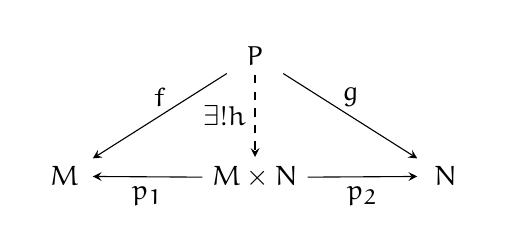
\begin{tikzpicture}
  \matrix (m) [matrix of math nodes,row sep=3em,column sep=4em,minimum width=2em]
  {
     & P &  \\
     M & M \times N & N \\};
  \path[-stealth]
    (m-1-2) edge node [above] {$f$} (m-2-1)
            edge [dashed] node [left] {$\exists ! h$} (m-2-2)
            edge node [above] {$g$} (m-2-3)
    (m-2-2) edge node [below] {$p_1$} (m-2-1)
    (m-2-2) edge node [below] {$p_2$} (m-2-3);
\end{tikzpicture}
\end{center}
\item[(c)] Si $p \in M$ y $(U, \varphi)$ es una carta de $M$ con $p \in U$, el siguiente diagrama
\begin{center}
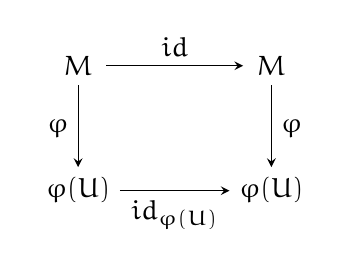
\begin{tikzpicture}
  \matrix (m) [matrix of math nodes,row sep=3em,column sep=4em,minimum width=2em]
  {
     M & M\\
     \varphi(U) & \varphi(U)\\};
  \path[-stealth]
    (m-1-1) edge node [above] {$id$} (m-1-2)
            edge node [left] {$\varphi$}  (m-2-1)
    (m-2-1) edge node [below] {$id_{\varphi(U)}$} (m-2-2)
    (m-1-2) edge node [right] {$\varphi$} (m-2-2);
\end{tikzpicture}
\end{center}
conmuta e $id_{\varphi(U)} = \varphi\varphi^{-1}$ es siempre diferenciable. Por lo tanto, $id$ es diferenciable y entonces por $\paint{purple}{(b)}$ existe una \'unica funci\'on $f : M \to M \times M$ tal que $p_1f = id = p_2f$, que resulta diferenciable. Como $\Delta$ cumple lo primero, debe ser $\Delta = f$ y por lo tanto, $\Delta$ es diferenciable.
\end{itemize}
\end{proof}
\end{document}
